\chapter{Elemente ale arhitecturii hardware}
\label{chap:hard}

\section{Diagrama de context}

Modul de func\c{t}ionare al sistemului este prezentat \^{i}n diagrama de context din   \figref{fig:diag.context}.

\begin{figure}[!ht]
    \begin{center}
    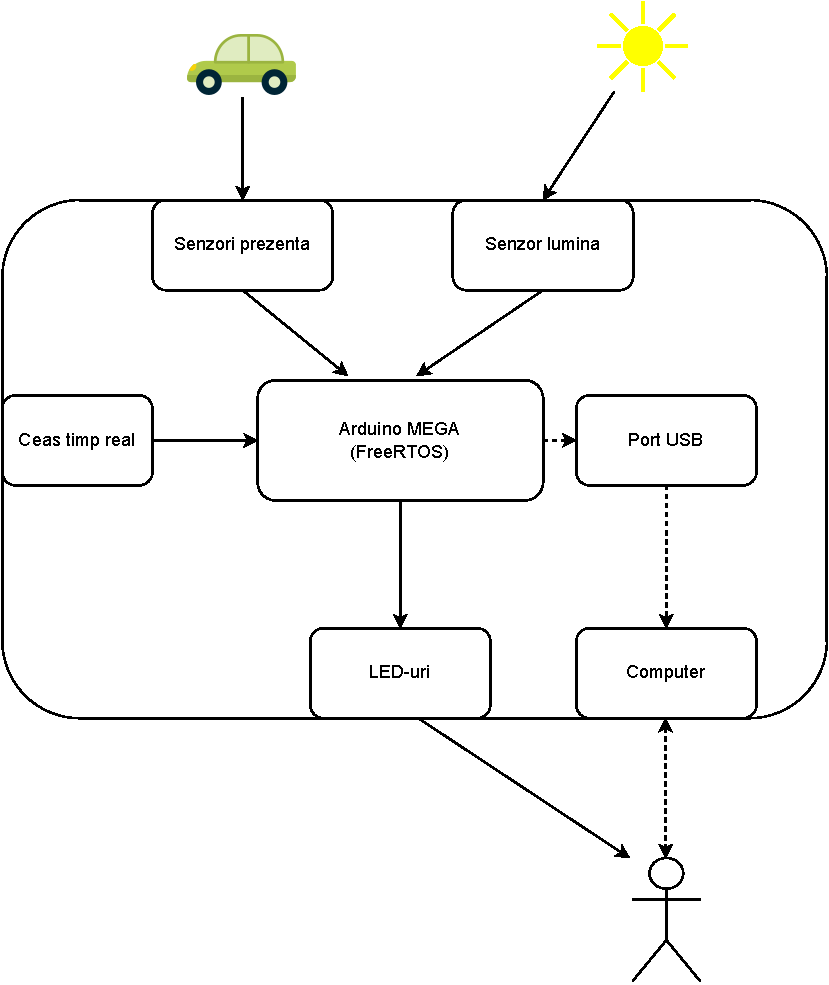
\includegraphics[width=0.7\linewidth,keepaspectratio]{pics/diag_context.drawio.pdf}
    \end{center}
    \caption{Diagrama de context a sistemului în timp real pentru monitorizarea iluminatului public}
    \label{fig:diag.context}
\end{figure}

Componentele sistemului \^{i}n timp real sunt urm\u{a}toarele, conform diagramei de context:

\begin{itemize}
  \item 5 module cu senzor infraroșu; 
\item 3 diode de tip LED;     
 \item Un fotorezistor de tip LDR 5528;
\item  Microcontroller Arduino Mega;
\item  Un ceas în timp real;
\item  Port USB; 
\item Computer.
\end{itemize}

\section{Prezentare elemente diagram\u{a} context}
\subsection{Modul senzor poziție} \label{senzorir}
 Am folosit 5 astfel de module HW-201, ilustrat în \figref{fig:IR1}, pentru detectarea prezenței vehiculelor de pe stradă. Acesta dispune și de un potențiometru, care permite ajustarea razei de detecție a obiectelor la valoarea dorită din intervalul 2-30 cm.

\begin{figure}[!ht]
    \centering
    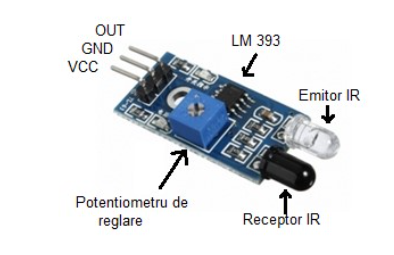
\includegraphics[width=0.4\linewidth,keepaspectratio]{pics/SenzorIR.jpg}
    \caption{Modul infraro\c{s}u}
    \label{fig:IR1}
\end{figure}

Elementul emițător eliberează constant un fascicul de lumină infraroșie, care se reflectă și ajunge la receptor atunci când există un obiect destul de aproape, după cum este prezentat în \figref{fig:IR2}. O mențiune legată de acest mod de funcționare este faptul că, la folosirea a 2 senzori pe părți opuse ale drumului, aceștia trebuie reglați din potențiometru pentru a avea raza de acțiune mai mică decât jumătate din lungimea drumului. În caz contrar, se vor activa reciproc.

\begin{figure}[!ht]
    \centering
    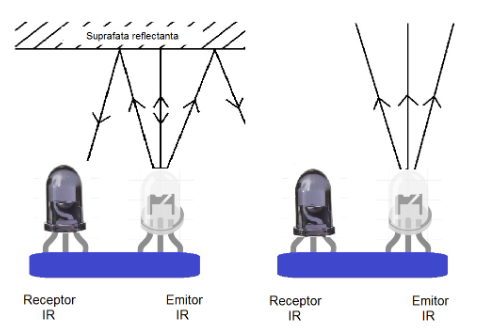
\includegraphics[width=0.6\linewidth,keepaspectratio]{pics/senzorIR2.jpg}
    \caption{Func\c{t}ionare modul infraro\c{s}u}
    \label{fig:IR2}
\end{figure}
O limitare a senzorilor ce se bazează pe detectarea radiațiilor infraroșii este că nu pot fi folosiți pe timp de zi fară a fi influențați negativ de lumina soarelui(e.g. se activează fără nimic în fața lor). Acest lucru nu afectează funcționarea dorită a sistemului, fiind luat în considerare că intrările de la acești senzori sunt citite doar noaptea, ci este doar un inconvenient la realizarea testării pe timp de zi.

În cazurile în care sunt alăturați 2 senzori, distanța dintre aceștia trebuie să fie destul de mare comparativ cu raza de detecție aleasă, pentru a nu permite activarea nedorită a unui senzor de reflecția fasciculului infraroșu al senzorului activat anterior, sau de cel de după el. O altă soluție este acoperirea parțială  a receptorului fiecărui senzor, pentru a permite doar detecția fasciculelor venite de la unghiuri mici, adică de la propriul emițător. 
\subsection{Fotorezistor}

Am ales acest element (\figref{fig:ldr}), pentru a diferenția între momentele când este zi sau noapte. Fotorezistorul este un tip de rezistență ce variază în funcție de gradul de luminozitate aplicat suprafeței acestuia. El este conectat în serie cu o rezistență fixă de 10k$\Omega$, iar valoarea analogică a tensiunii măsurate pe acest rezistor este convertită de Arduino Mega într-un număr natural din intervalul [0,1024]. Compararea acestei valori cu o constantă aleasă arbitrar va determina separarea între cele două moduri de funcționare.

\begin{figure}[!ht]
    \begin{center}
    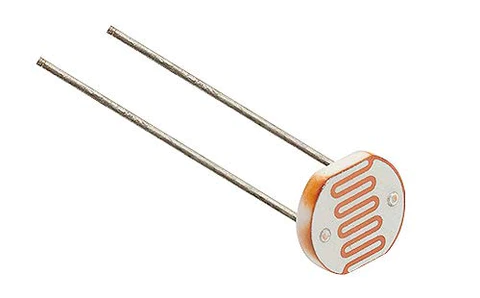
\includegraphics[width=0.3\linewidth,keepaspectratio]{pics/LDR.jpg}
    \end{center}
    \caption{Fotorezistor}
    \label{fig:ldr}
\end{figure}



\subsection{LED-uri}

Am folosit 3 diode de tip LED pentru simularea felinarelor în realizarea proiectului. Am conectat în serie câte o rezistență de 220 $\Omega$ la anodul fiecăreia dintre ele. 

\subsection{Arduino Mega} \label{mega}

Placa de dezvoltare Arduino Mega, ilustrată în \figref{fig:mega}, realizează calculele necesare funcționării corespunzătoare a sistemului. Aceasta dispune și de un ceas în timp real, care va fi util pentru dezvoltarea aplicației folosite. 

\begin{figure}[!ht]
    \begin{center}
    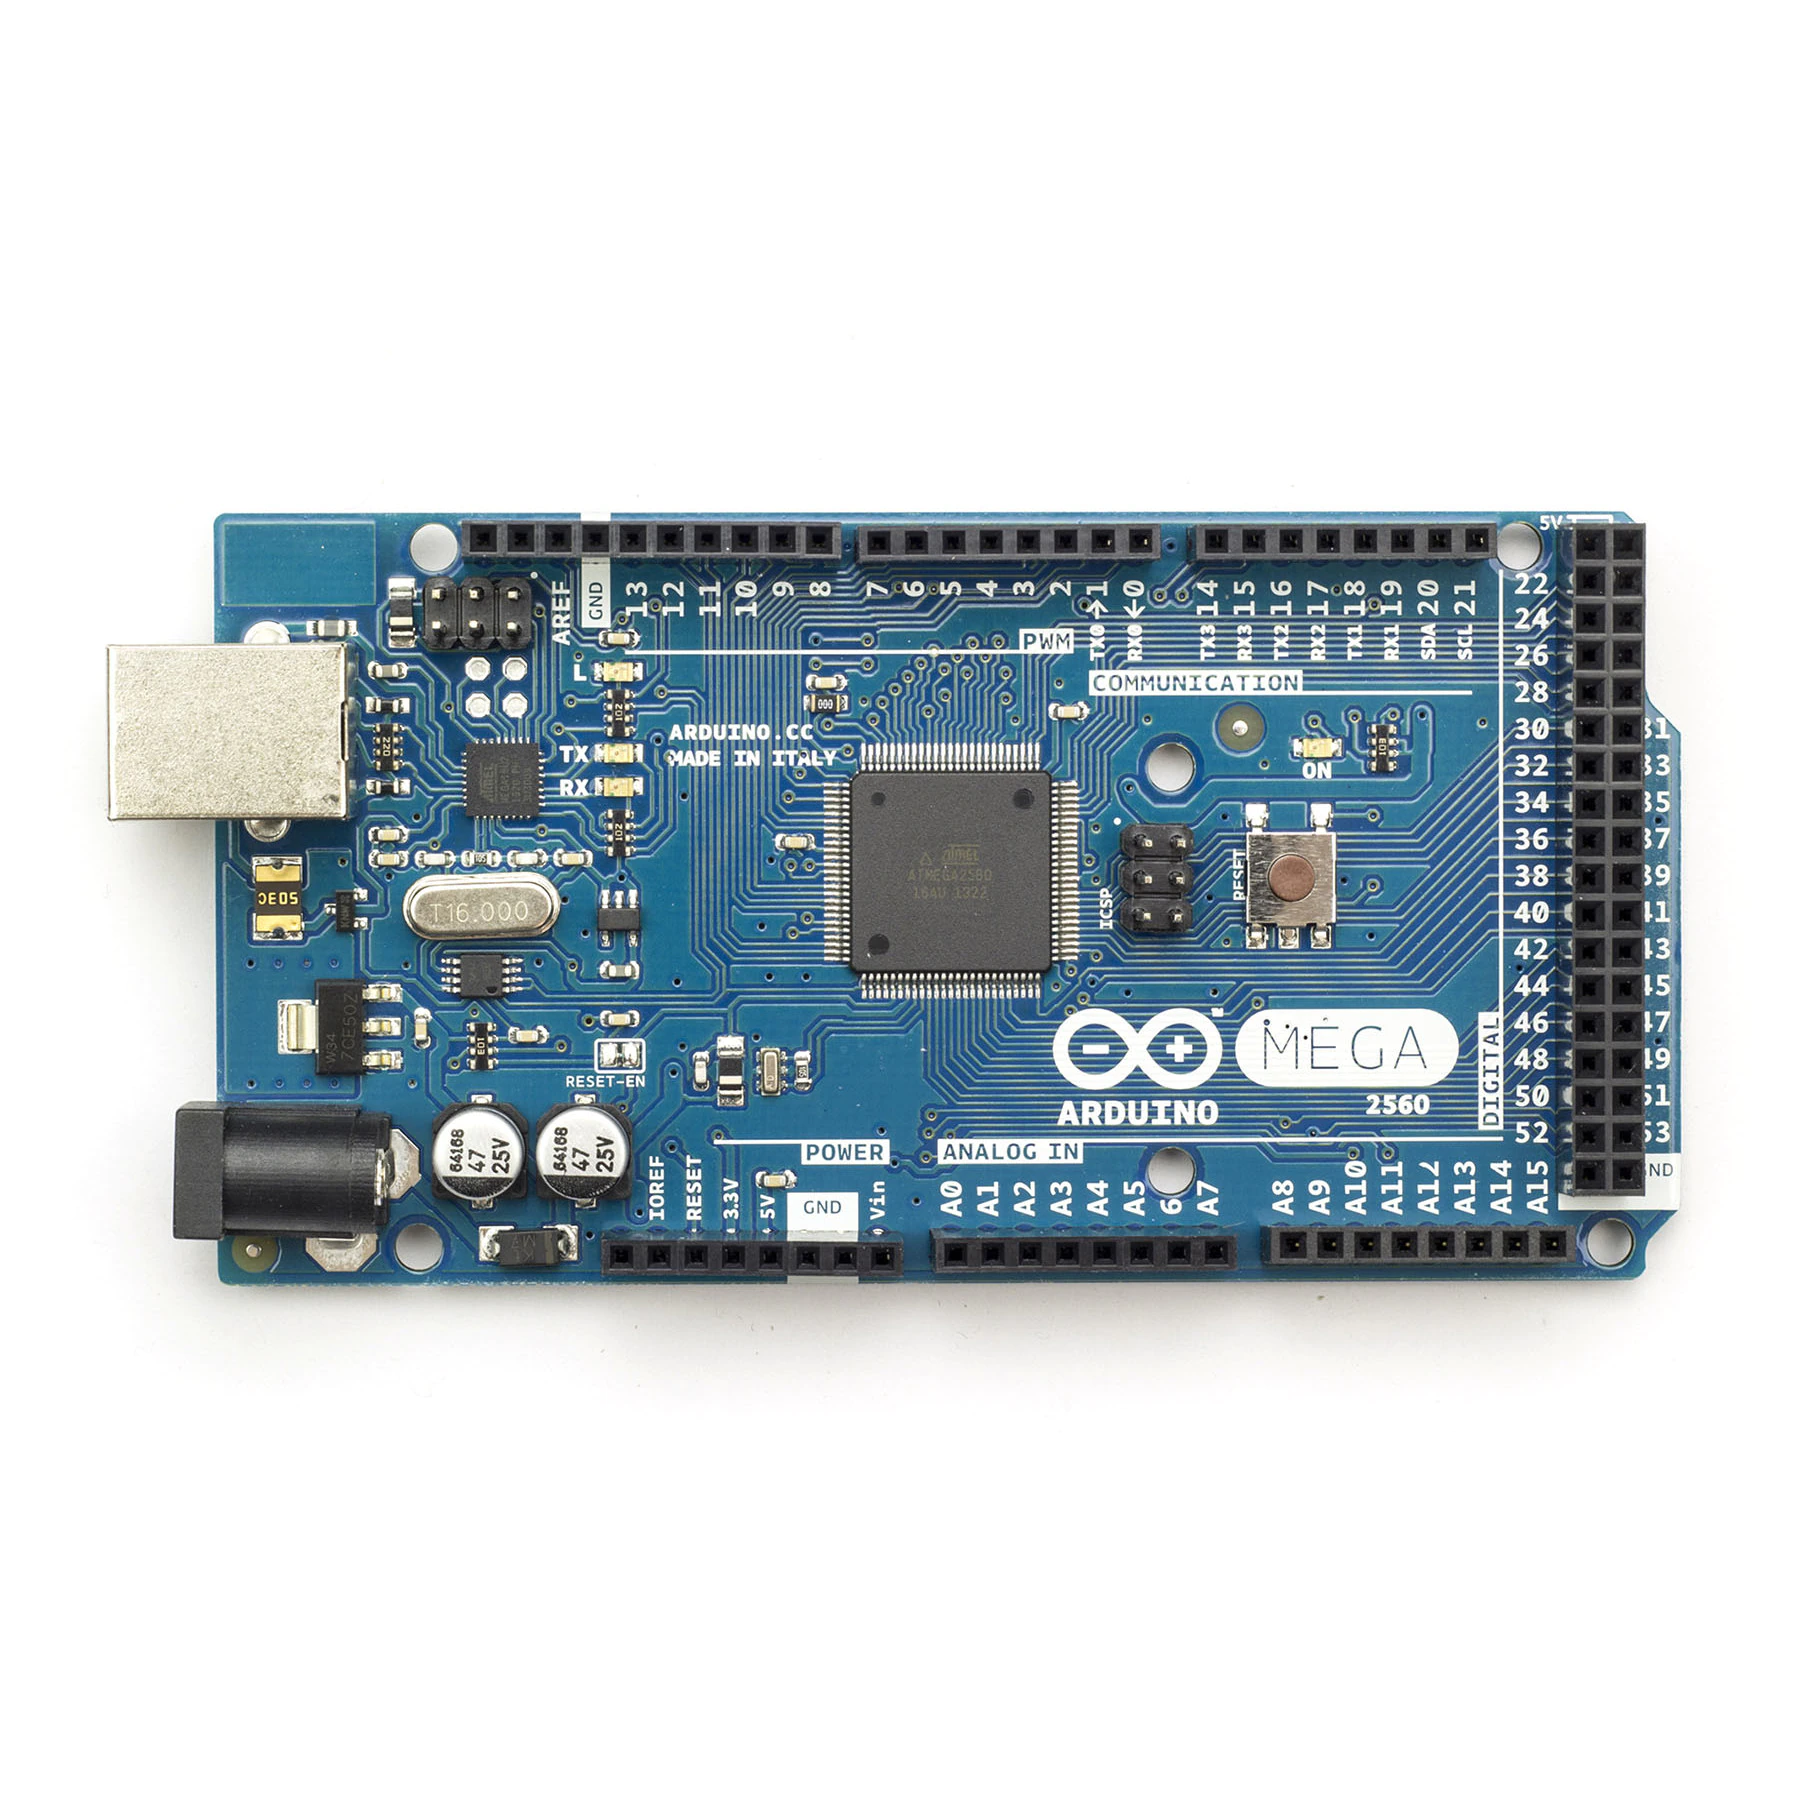
\includegraphics[width=0.5\linewidth,keepaspectratio]{pics/mega.jpg}
    \end{center}
    \caption{Microcontroller Arduino Mega}
    \label{fig:mega}
\end{figure}

Timpul este măsurat cu ajutorul unui ceas oscilator ce generează semnale dreptunghiulare cu frecvența, în cazul unui microcontroller Arduino, de 16MHz. Numărarea repetărilor acestui semnal duce la determinarea cu acuratețe a intervalelor de timp, până la dimensiuni de $\mu$s, conform \cite{Smythe2021.8} .Tot prin microcontroller se realizează și posibila conexiune cu un computer. Cel din urmă nu este strict necesar pentru funcționarea sistemului, dar cu ajutorul său se deschide accesul la citirea de către utilizator a datelor de la senzori și la modificarea codului sursă. Poate fi înlocuit cu o baterie sau altă sursă cu tensiunea recomandată între 7-12V DC.

Deși nu dispune de ieșiri analogice, 15 dintre pinii digitali de pe Arduino Mega permit utilizarea de \gls{pwm}. Această metodă permite transmiterea parțială a curentului la LED-uri, prin mijloace digitale. Alternarea între valori de 0 și 1 creează un semnal dreptunghiular, iar controlul duratei impulsului acesta permite simularea unui semnal analogic \cite{Smythe2021.7}. Această metodă va permite controlul intensității luminii felinarelor.




\section{Simulare a sistemului în Tinkercad și realizarea fizică}



În \figref{fig:arduino} este reprezentată o schemă a modului de conectare a componentelor descrise mai devreme, realizată de mine în Tinkercad. Este de menționat faptul că această platformă nu dispune de toate piesele necesare. Prin urmare, am înlocuit placa Arduino Mega cu un Arduino UNO, iar senzorii de prezență sunt reprezentați printr-o versiune ce dispune doar de receptor. În schimb, modul de conectare va rămâne același și pentru componentele ce au fost schimbate, doar pinii digitali folosiți pentru conectarea senzorilor vor varia față de modelul meu.

\begin{figure}[!ht]
    \begin{center}
    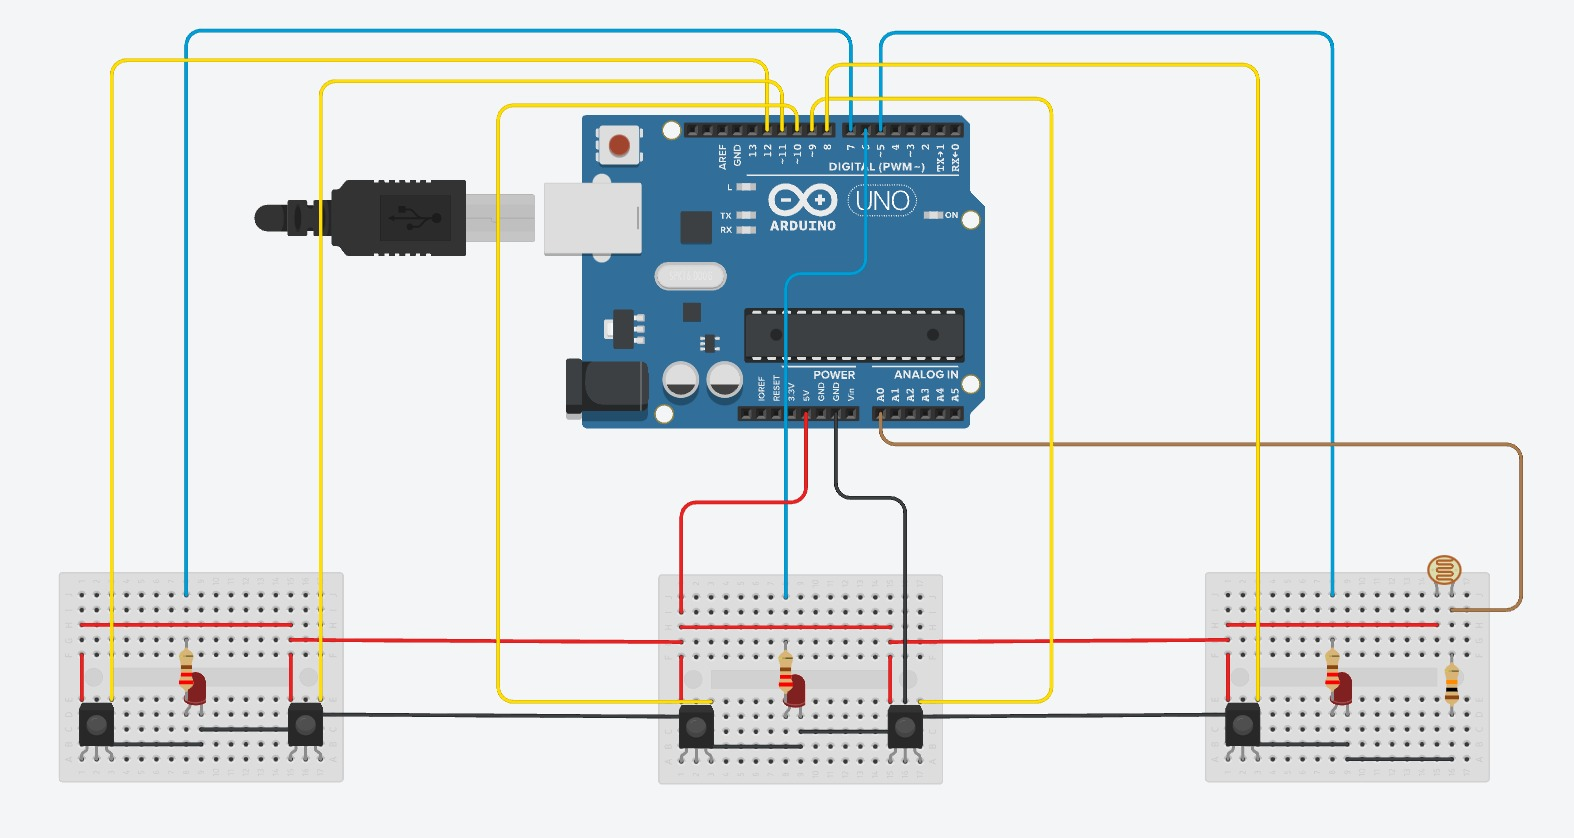
\includegraphics[width=\linewidth,keepaspectratio]{pics/Schema_Arduino.jpg}
    \end{center}
    \caption{Schema sistemului, realizată în Tinkercad}
    \label{fig:arduino}
\end{figure}


Toate componentele sunt conectate la pinul GND, iar senzorii de prezență și fotorezistorul sunt conectați și la pinul de alimentare cu 5V. Citirea datelor se va face pe pinii digitali 49, 50, 51, 52, 53 (8, 9, 10, 11, 12 în \figref{fig:arduino}), de pe Arduino Mega, pentru senzorii de prezență și de la pinul pentru intrări analogice A0 pentru fotorezistor. Intensitatea cu care se vor aprinde LED-urile va fi transmisă pe pinii digitali 5, 6, 7, prin \gls{pwm}.

În \figref{fig:model} este modelul realizat de mine, conform schemei prezentate anterior. Acoperirea   acestuia ajută la blocarea parțială a luminii soarelui la testarea pe timp de zi, iar spațiul lăsat liber permite accesul unui cablu de alimentare la microcontroller. Distanța dintre doi senzori consecutivi este $d=14$cm, egală cu cea dintre 2 felinare consecutive. Poziția fotorezistorului, în partea stângă a modelului, a fost aleasă pentru ca valoarea citită de la acesta să fie influențată cât mai puțin de aprinderea LED-urilor.

\begin{figure}[!ht]
    \begin{center}
    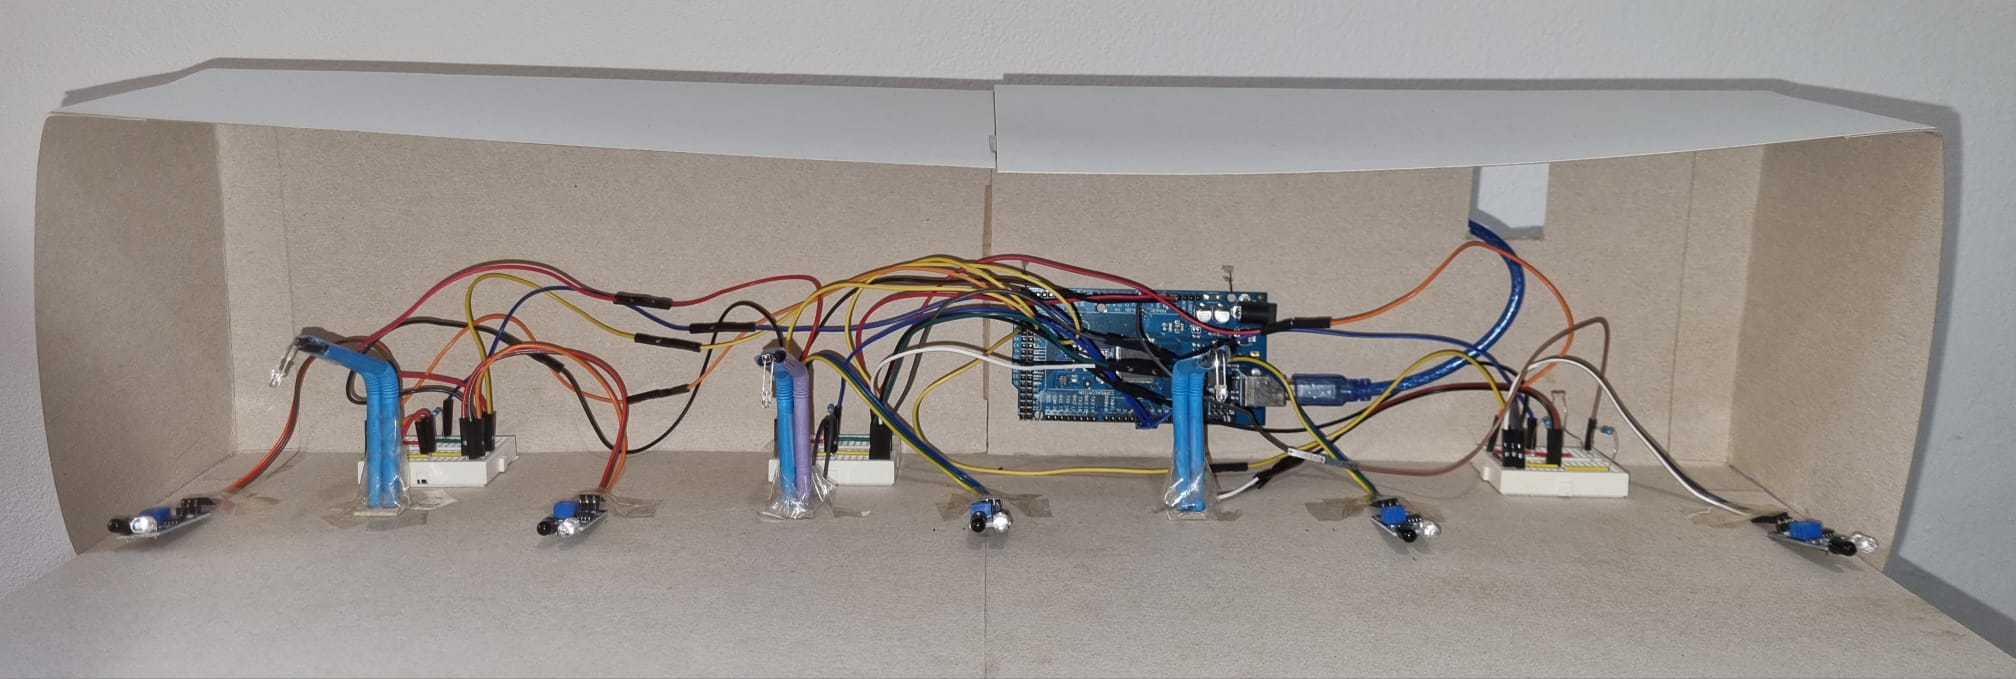
\includegraphics[width=\linewidth,keepaspectratio]{pics/sistemirl.jpeg}
    \end{center}
    \caption{Modelul implementat în realitate}
    \label{fig:model}
\end{figure}